% DriftWatch paper. IEEE conference template (IEEEtran), A4, as used by IEEE EuroS&P.
% Every number comes from docs/CLAIMS.md and carries its claim id in small type, e.g. {\clm{E-30}}.
% Build: tectonic paper/main.tex   (or any LaTeX with IEEEtran and BibTeX)
\documentclass[conference,a4paper]{IEEEtran}
\usepackage[T1]{fontenc}
\usepackage[utf8]{inputenc}
\usepackage{microtype}
\usepackage{booktabs}
\usepackage{graphicx}
\usepackage{amsmath}
\usepackage{tikz}
\usetikzlibrary{arrows.meta,positioning,calc}
\usepackage{url}
\usepackage[hidelinks]{hyperref}
\newcommand{\clm}[1]{{\scriptsize[#1]}}
\newcommand{\aaut}{A-AUT}

\ifdefined\anonymous\newcommand{\anonif}[2]{#1}\else\newcommand{\anonif}[2]{#2}\fi
\begin{document}

\title{Detector Lifetime Under Delayed Labels:\\
A Pre-Registered Time-Aware Study on Android and Windows PE Malware}

\author{\anonif{\IEEEauthorblockN{Anonymous submission}}{\IEEEauthorblockN{Yathindra K B}
\IEEEauthorblockA{VISTAS, India\\
yathindrakb25@gmail.com}}}

\maketitle

\begin{abstract}
A malware detector decays as malware changes, and an analyst team can slow the decay only by labelling samples that arrive late and are limited in number. We study malware detector lifetime under label delay, a fixed analyst budget and conformal drift monitoring in a single time-aware protocol, reported with A-AUT, on Android and Windows PE data. The protocol enforces the three TESSERACT constraints as assertions that raise, simulates a label queue in which no policy, selector or monitor can read a held-back label, and was pre-registered before the results of each of three grids (54, 56 and 76 cells) were produced. On two public feature datasets (LAMDA and BODMAS) and two detectors, we find small effects: retraining on bought labels helps a little on LAMDA, late labels cost a little, selecting labels by uncertainty or credibility is above random selection by about one to two hundredths of A-AUT, and no drift monitor beats retraining every third slot. Where a result depends on a choice, such as the random-split comparator, we report both readings. Code, claims ledger and registrations are public; every reported number maps to a file and a commit.
\end{abstract}

\begin{IEEEkeywords}
malware detection, concept drift, label delay, active learning, conformal prediction, time-aware evaluation, reproducibility
\end{IEEEkeywords}

\section{Introduction}
A learned malware detector is trained on yesterday's samples and used on tomorrow's. Its F1 score falls as the samples change, and the standard remedy is to retrain on newly labelled data. Two facts make this harder than the textbook picture. First, labels are not free: an analyst team can label only a limited number of samples per day. Second, labels are not instant: a sample queried today may receive its label days or weeks later. How long a detector stays useful therefore depends on three things at once, the delay, the budget and the rule that decides when and what to label.

Prior work evaluates these ingredients separately: time-aware experiment design and the AUT metric~\cite{pendlebury2019tesseract,kan2024tesseractext,chow2025beyond}, conformal drift detection~\cite{barbero2022transcending}, retraining under a labelling budget~\cite{chen2023continuous,amalapuram2026seed}, and the effect of label delay~\cite{botacin2025labeldelays}. This paper puts them into one protocol and one codebase. We state the claim as narrowly as we can:

\begin{quote}
\emph{We study malware detector lifetime under label delay, a fixed analyst budget and conformal drift monitoring in a single time-aware protocol, reported with A-AUT, on Android and Windows PE data.}
\end{quote}

This is a statement of what was measured, not of priority. The search behind it was limited, and neighbouring work covers subsets of the same ingredients.

\textbf{Research questions.} RQ1: how far does a random split overstate the time-aware score? RQ2: what do delay and budget cost or buy, and is the budget response concave? RQ3: does selecting labels by uncertainty or conformal credibility beat random selection, and does the advantage shrink under delay? RQ4: does a drift monitor that triggers retraining beat retraining on a fixed period at the same label cost?

\textbf{Contributions.}
(1)~A protocol with C1--C3, label delay and analyst budget as code, with a leakage canary and a mutation matrix in which all 15 deliberately broken constraints are caught~\clm{W-07}.
(2)~A simulator in which label delay lives in one module and held-back labels are sealed from selectors, policies and monitors, pinned by a spy test.
(3)~Three pre-registered grids, run to completion without a failed cell, with every decision made before or after the results marked as such.
(4)~A set of small or null effects, stated with intervals, and the audit trail behind each number.
We make no claim that a better detector results.

\section{Background}
\textbf{Time-aware evaluation.} TESSERACT~\cite{pendlebury2019tesseract} identifies spatial and temporal bias and proposes three constraints: C1, never train on the future; C2, evaluate each slot using only samples from that slot; C3, keep a realistic malware ratio in the test set. AUT is the normalised area under the F1-versus-time curve. The extended version~\cite{kan2024tesseractext} adds case studies in Windows PE and PDF, and Chow et al.~\cite{chow2025beyond} show that factors beyond these constraints still cause discrepancies and recommend reporting AUT over rolling windows (A-AUT), which we do.

\textbf{Drift and conformal monitors.} Conformal evaluation turns a classifier's score into a p-value relative to a calibration set and uses it to detect drift in malware classification~\cite{barbero2022transcending}. Its guarantees assume exchangeable samples~\cite{shafer2008tutorial}, which a drifting stream violates, and the label-conditional p-values need labels that a delay queue releases late.

\textbf{Retraining under a budget and under delay.} Continuous and active learning reduce the cost of keeping Android detectors current~\cite{chen2023continuous,minnei2026labelefficient,amalapuram2026seed}. Botacin and Gomes study label delays in detection pipelines and show that analysis-queue limits leave a large exposure~\cite{botacin2025labeldelays}; their figures come from their setting and none is reused here.

\textbf{Neighbours on drift, selection and delay.} Gama et al.\ frame concept drift as a change in the relation between inputs and target~\cite{gama2014survey}, and Ceschin et al.\ argue that drift, evolution, delayed labels and adversarial pressure must be treated together in security~\cite{ceschin2023stream}. For Windows PE, Li et al.\ study adaptation to real drifted malware from minimal samples~\cite{li2024revisiting}; for Android, DREAM and TIF address drift by explanation-based adaptation and by learning temporally invariant features~\cite{he2024dream,zheng2025tif}. ActDroid treats Android detection as an active online problem~\cite{muzaffar2024actdroid}, ADAPT lowers the labelling cost of frequent retraining by pseudo-labelling~\cite{alam2025adapt}, and DRMD learns to reject samples for manual labelling~\cite{mcfadden2026drmd}. Cerqueira et al.\ benchmark 14 drift detection methods on seven real-world datasets with timing-aware criteria~\cite{cerqueira2026driftbench}, which is the way our monitors are scored (alarm precision, recall and delay against drop events defined from true labels). We report these works at the level of their abstracts; none of their figures is reused, and we do not claim that the combination studied here is absent from the literature.

\section{Protocol}
\subsection{Data}
We use pre-extracted feature files only; no sample is downloaded, executed or redistributed. LAMDA~\cite{haque2025lamda} is an Android dataset of 1,008,381 apps in Drebin-style sparse features; its month comes from the AndroZoo \texttt{added} date, and its labels follow a VirusTotal rule (no detection is benign, four or more is malware, one to three are discarded)~\clm{D-15}. BODMAS~\cite{yang2021bodmas} holds 57,293 malware and 77,142 benign Windows PE files in 2,381-dimensional EMBER-style features over about thirteen months. Time is cut into equal slots by first-seen date: a month for LAMDA, two weeks for BODMAS.

\begin{table}[t]
\centering
\caption{The two datasets as used (feature files only).}
\label{tab:data}
\small
\begin{tabular}{@{}lll@{}}
\toprule
 & LAMDA & BODMAS\\
\midrule
Platform & Android & Windows PE\\
Period & 2013 to 2025 & Aug 2019 to Sep 2020\\
Samples & 1,008,381 & 57,293 mal., 77,142 ben.\\
Features & Drebin-style, sparse & 2,381, EMBER-style\\
Slot & one month & two weeks\\
Licence & MIT & code BSD-2-Clause$^{a}$\\
Windows in E2 & 16 \clm{E-28} & 20 distinct slots \clm{E-12}\\
\bottomrule
\end{tabular}

\smallskip
\raggedright\scriptsize $^{a}$ The dataset files carry no stated licence; they are used as published and not redistributed.
\end{table}

\subsection{Slots, windows and constraints}
A window trains on the first slots and then steps through the following evaluation slots one at a time; the window geometry is fixed by an ADR before any grid. C1 and C2 are checked by assertions that raise on violation, and C3 subsamples malware to a fixed 10\% ratio per slot (with a cap-and-flag rule when a slot has too little malware), with a sensitivity check at another ratio. A slot that already has less malware than the target keeps all its rows and is flagged rather than dropped; 31 of the 62 LAMDA headline months are below 10\% malware.~\clm{W-01}

\subsection{Metric}
For per-slot F1 values $f_1,\dots,f_N$, $\mathrm{AUT}=\frac{1}{N-1}\sum_{k=1}^{N-1}\frac{f_k+f_{k+1}}{2}$. A-AUT is the mean and standard deviation of AUT over rolling windows. We state intervals as two-stage bootstrap percentile intervals: moving blocks of windows, then seeds within windows, 10,000 replicates~\clm{P-08}. A contrast is \emph{detected} when its 95\% interval excludes zero in the hypothesised direction, and \emph{equivalent} when the whole interval lies within $\pm0.01$ of A-AUT~\clm{P-10}.

\subsection{Delay, budget, policies, selectors, monitors}
\textbf{Delay and budget.} A sample queried in slot $t$ is usable for training from slot $t+1+d$, with $d\in\{0,1,2,3\}$. The budget is 0.5, 1, 2 or 5\% of the slot, and we always report the absolute count next to the percentage.
\textbf{Policies.} \emph{Never} trains once; \emph{periodic} retrains every third slot; \emph{monitor-triggered} retrains when a monitor alarms. Retraining uses only labels that have arrived.
\textbf{Selectors.} \emph{Random}; \emph{uncertainty} (closest to 0.5); \emph{credibility} (lowest Mondrian conformal p-value). A random slice is reserved for calibration.
\textbf{Monitors.} Four label-free monitors behind one alarm interface: a Kolmogorov--Smirnov test on top features, MMD, a domain classifier, and a p-uniformity test on conformal scores.
\textbf{Detectors.} Logistic regression and LightGBM at fixed hyperparameters; the point is the protocol, not a better detector.

\section{Simulator and assurance}
\begin{figure}[t]
\centering
\begin{tikzpicture}[
  node distance=4mm and 5mm,
  box/.style={draw, rounded corners=1.5pt, align=center, font=\scriptsize, minimum height=6.5mm, inner sep=2pt},
  sealed/.style={box, fill=black!10},
  >={Stealth[length=1.6mm]}, font=\scriptsize]
  \node[box] (slot) {slot $t$\\(features only)};
  \node[box, right=of slot] (score) {score slot $t$\\(before any query)};
  \node[box, right=of score] (sel) {selector\\policy, monitor};
  \node[sealed, below=of sel] (queue) {label queue\\release at $t{+}1{+}d$};
  \node[sealed, left=of queue] (truth) {true labels\\(sealed)};
  \node[box, below=of slot] (pool) {training pool\\(arrived labels)};
  \draw[->] (slot) -- (score);
  \draw[->] (score) -- (sel);
  \draw[->] (sel) -- node[right, font=\tiny]{queries} (queue);
  \draw[->] (truth) -- (queue);
  \draw[->] (queue.south) -- ++(0,-3mm) -| node[pos=0.25, below, font=\tiny]{released labels} (pool.south);
  \draw[->] (pool.north) -- node[left, font=\tiny]{retrain} (slot.south);
\end{tikzpicture}
\caption{One slot of the simulator. Selectors, policies and monitors see only the features of the slot; the queue is the only module that applies a delay and the only reader of true labels besides the scorer.}
\label{fig:sim}
\end{figure}

\textbf{Sealed labels.} Label delay lives only in the queue module. A label queried in slot $t$ is released exactly once, ignored and counted if its release slot falls after the evaluation window, and never readable before then; tests cover $d\in\{0,1,2,3\}$ and 150 property-based scenarios~\clm{S-01}. Selectors, policies and monitors receive an opaque view of a slot; a spy test and a label-invariance test show they cannot reach a held-back label. A slot is scored before any label queried in it can exist.

\textbf{Mutation checks.} We broke the slicer and constraints in 15 documented ways (for example one training sample as new as the test slot, shuffled timestamps, an inclusive end of the slot window) and confirmed that the real test suites catch every one~\clm{W-07}. This is a check of code behaviour, not evidence about detectors. A leakage canary shows AUT moving toward the random-split score when leakage is planted in seeded drift.

\textbf{Reproducibility.} Every run has one YAML configuration; its hash covers the config, the code version and the lock file. Per-slot predictions are stored. A smoke experiment on a synthetic fixture runs from an installed wheel, and \texttt{driftwatch reproduce table1} reproduces the first table on BODMAS: on a clean tree the time-aware columns matched to four decimals~\clm{E-24,E-82}.

\section{Experiments and pre-registration}
Experiments E0 to E4 were run, and three of them were pre-registered. E0 and E1 (baselines and the label-influence diagnostic) were run and read \emph{before} the first registration, so RQ1 is a registered reading of numbers already known, and its primary comparator was chosen after both numbers were seen~\clm{E-18}. E2 (delay $\times$ budget, 54 cells) was registered under tag \texttt{prereg-v1}, E3 (selection under delay, 56 cells) under \texttt{prereg-v2}, and E4 (drift monitors, 76 cells) under \texttt{prereg-v3}, each before its first result. All 186 cells completed and none failed~\clm{E-26,E-40,E-48}. Seeds extended after reading (LAMDA seeds 5 to 9 of E3) and one setting stated after the results (the Holm floor of E4) are marked as such in the registrations and in the claims ledger~\clm{P-18}. E5 (cross-platform repeat) and E6 (EMBER2024) were not run.

\section{Results}
We report A-AUT differences with 95\% intervals; standard deviations over LAMDA windows are 0.050 to 0.069~\clm{E-28}. Figure~\ref{fig:e2} shows the per-slot curves and Table~\ref{tab:main} gathers the headline contrasts.

\begin{figure*}[t]
\centering
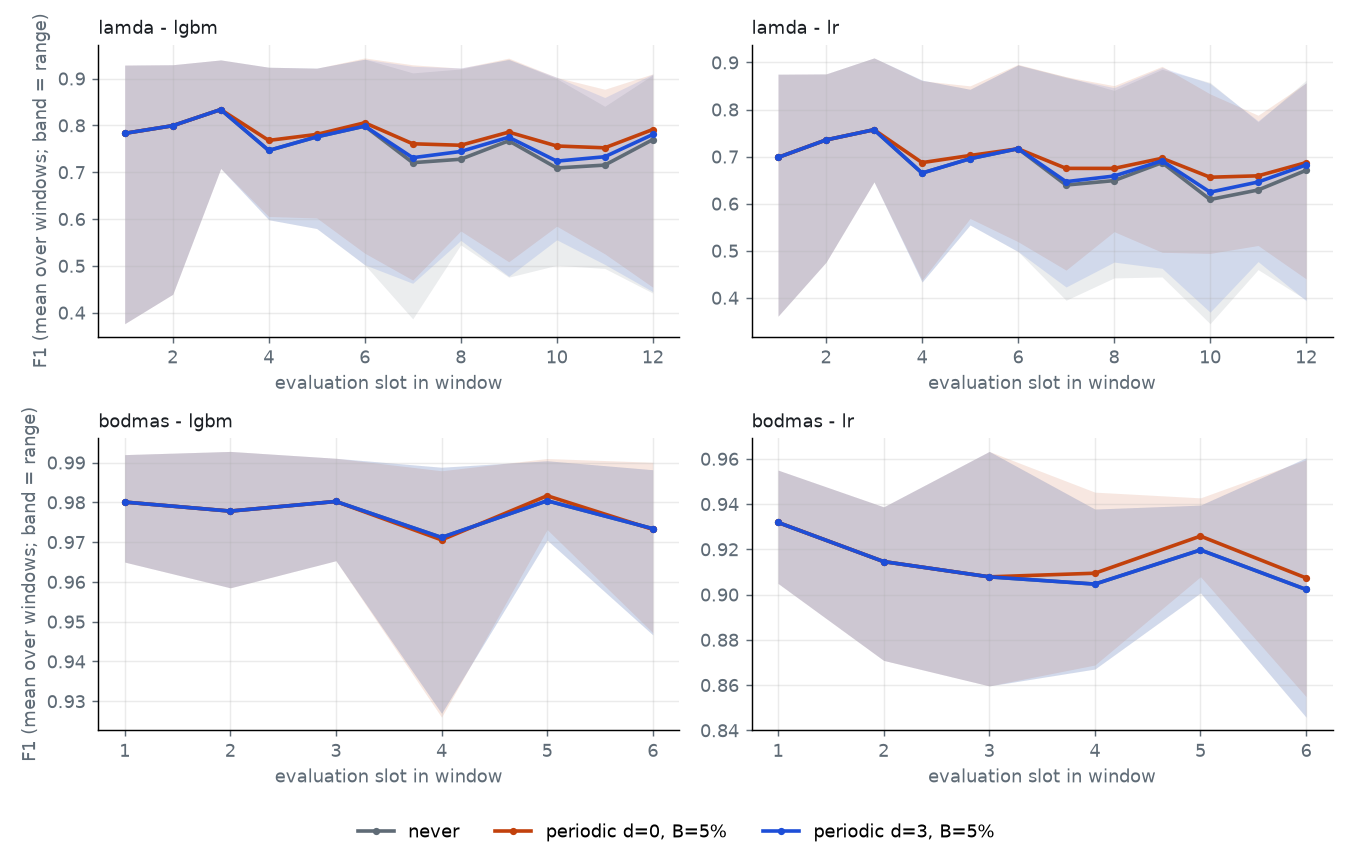
\includegraphics[width=0.78\textwidth]{../reports/figures/e2_per_slot_curves.png}
\caption{E2: per-slot F1 inside a window (mean over windows, band is the range over windows) for never retraining, periodic retraining with no delay and periodic retraining with a delay of three slots, both at 5\% of the slot \clm{E-26}. On LAMDA the never-retrained curve falls below the retrained ones from about the fourth evaluation slot; on BODMAS they are almost the same.}
\label{fig:e2}
\end{figure*}

\begin{table}[t]
\centering
\caption{Headline contrasts, A-AUT difference with 95\% interval (LAMDA unless stated). LR is logistic regression, LGBM is LightGBM.}
\label{tab:main}
\small
\begin{tabular}{@{}p{3.15cm}ll@{}}
\toprule
Contrast & LR & LGBM\\
\midrule
Periodic minus never, $d{=}0$, 5\% \clm{E-30} & 0.017 [0.007, 0.024] & 0.020 [0.012, 0.022]\\
Delay 0 minus delay 3, 5\% \clm{E-30} & 0.011 [0.005, 0.017] & 0.013 [0.008, 0.015]\\
Periodic minus never, BODMAS \clm{E-29} & 0.003 & none\\
Selection over random, $d{=}0$ \clm{E-43} & \multicolumn{2}{c}{0.0109 to 0.0177}\\
Selection over random, $d{=}3$ \clm{E-43} & \multicolumn{2}{c}{0.0015 to 0.0095}\\
Selection $\times$ delay interaction \clm{E-42} & \multicolumn{2}{c}{0.0061 to 0.0118 (8 of 8 positive)}\\
\bottomrule
\end{tabular}
\end{table}

\textbf{RQ2: delay and budget.} Periodic retraining with 5\% of each month's samples labelled (about 218 labels per slot) is above never retraining by 0.017 [0.007, 0.024] for logistic regression and 0.020 [0.012, 0.022] for LightGBM; on BODMAS the difference is 0.003 for logistic regression and none for LightGBM~\clm{E-30,E-29}. A delay of three slots instead of zero costs 0.011 and 0.013 at 5\%; at 1\% the cost is not detected for logistic regression and lies inside the 0.01 margin for LightGBM. Moving from 0.5\% to 5\% adds 0.013 and 0.017 on LAMDA. Diminishing returns are detected in one stratum of four: per 100 extra labels per slot the gain falls from 0.017 to 0.007 for LAMDA LightGBM~\clm{E-34}. Whether the delay cost grows with budget was not a registered contrast and is not claimed. On BODMAS there is one useful refit per window, so at $d=3$ periodic retraining equals never retraining by construction and its delay numbers measure a delay in a single refit~\clm{P-12}.

\begin{table}[t]
\centering
\caption{E2 on LAMDA: A-AUT(F1), mean over 16 windows (sd over windows), five seeds, periodic retraining, mean labels per slot \clm{E-28}.}
\label{tab:e2}
\small
\begin{tabular}{@{}lccc@{}}
\toprule
Arm & Labels/slot & LR & LGBM\\
\midrule
never & 0 & 0.679 (0.058) & 0.760 (0.069)\\
$d{=}0$, 0.5\% & 21.8 & 0.682 (0.058) & 0.763 (0.068)\\
$d{=}0$, 1\% & 43.6 & 0.683 (0.058) & 0.767 (0.066)\\
$d{=}0$, 2\% & 87.3 & 0.687 (0.055) & 0.772 (0.064)\\
$d{=}0$, 5\% & 218.3 & 0.694 (0.050) & 0.781 (0.059)\\
$d{=}3$, 5\% & 218.3 & 0.684 (0.054) & 0.767 (0.065)\\
\bottomrule
\end{tabular}
\end{table}

\textbf{RQ1: the random-split gap.} Under the registered per-slot comparator the gap is 0.03 to 0.04 on LAMDA and 0.006 to 0.035 on BODMAS, below the registered 0.05 band, while the LAMDA LR interval still contains 0.05; under the window-level comparator it is 0.14 to 0.15 on LAMDA~\clm{E-35}. The two readings differ because of how the comparator matches class counts, and the primary one is biased downwards on LAMDA~\clm{E-18}. We therefore do not claim that the gap is caused by temporal leakage alone.

\textbf{RQ3: selection.} On LAMDA, with ten seeds and 43.6 and 87.3 labels per slot, uncertainty or credibility selection is above random selection at equal labels by 0.0109 to 0.0177 with no delay and 0.0015 to 0.0095 after a delay of three slots; at $d=3$ three of eight advantages, all logistic regression, have intervals that include zero~\clm{E-43}. The interaction is positive in all eight rows, 0.0061 to 0.0118, under a Wilcoxon test on seed means that is conditional on the realised windows~\clm{E-42}. The advantage is not separated from a change in class mix of the labels that arrive~\clm{E-47}, and we do not show that credibility adds anything over uncertainty. The calibration-contaminated trap arm never retrains, so it is not read as evidence about contamination~\clm{E-45}.

\begin{table}[t]
\centering
\caption{E3 on LAMDA at $d{=}0$, 2\% budget, seeds 0 to 4: share of malware among the labels that arrived, and A-AUT, by selector \clm{E-47}.}
\label{tab:e3}
\small
\begin{tabular}{@{}lcccc@{}}
\toprule
 & \multicolumn{2}{c}{LR} & \multicolumn{2}{c}{LGBM}\\
\cmidrule(lr){2-3}\cmidrule(lr){4-5}
Selector & malware & A-AUT & malware & A-AUT\\
\midrule
random & 0.085 & 0.6676 & 0.085 & 0.7647\\
credibility & 0.193 & 0.6829 & 0.303 & 0.7806\\
uncertainty & 0.266 & 0.6870 & 0.401 & 0.7812\\
\bottomrule
\end{tabular}
\end{table}

\textbf{RQ4: monitors.} None of the 32 monitor-minus-periodic contrasts has an interval above zero; logistic regression with the KS monitor is below periodic retraining by 0.0089 [$-$0.0225, $-$0.0002] at $d=0$ and 0.0052 [$-$0.0136, $-$0.0007] at $d=3$ on LAMDA, a descriptive reading without family-wise control~\clm{E-59,E-60,P-18}. At the same number of refits the timing of the alarms made no difference larger than 0.01 on LAMDA~\clm{E-61}, but the monitors alarmed in most slots, so where an alarm fires every slot the matched control does not test timing~\clm{E-63}. This is a negative result at one budget and one frozen alarm level.

\begin{table}[t]
\centering
\caption{E4 monitor quality on LAMDA with LightGBM, monitors observing the never-retrained arm: alarm rate, alarm precision (95\% interval) against the precision of alarming in every slot (0.443), and alarm recall, for drops of at least 0.05 below the trailing three-slot mean \clm{E-63}.}
\label{tab:e4}
\small
\begin{tabular}{@{}lccc@{}}
\toprule
Monitor & Alarm rate & Precision & Recall\\
\midrule
KS (top features) & 0.617 & 0.462 [0.354, 0.546] & 0.743\\
MMD & 0.796 & 0.449 [0.328, 0.546] & 0.942\\
Domain classifier & 0.997 & 0.444 [0.327, 0.529] & 1.000\\
p-uniformity & 0.562 & 0.461 [0.315, 0.555] & 0.796\\
\bottomrule
\end{tabular}
\end{table}

\begin{figure*}[t]
\centering
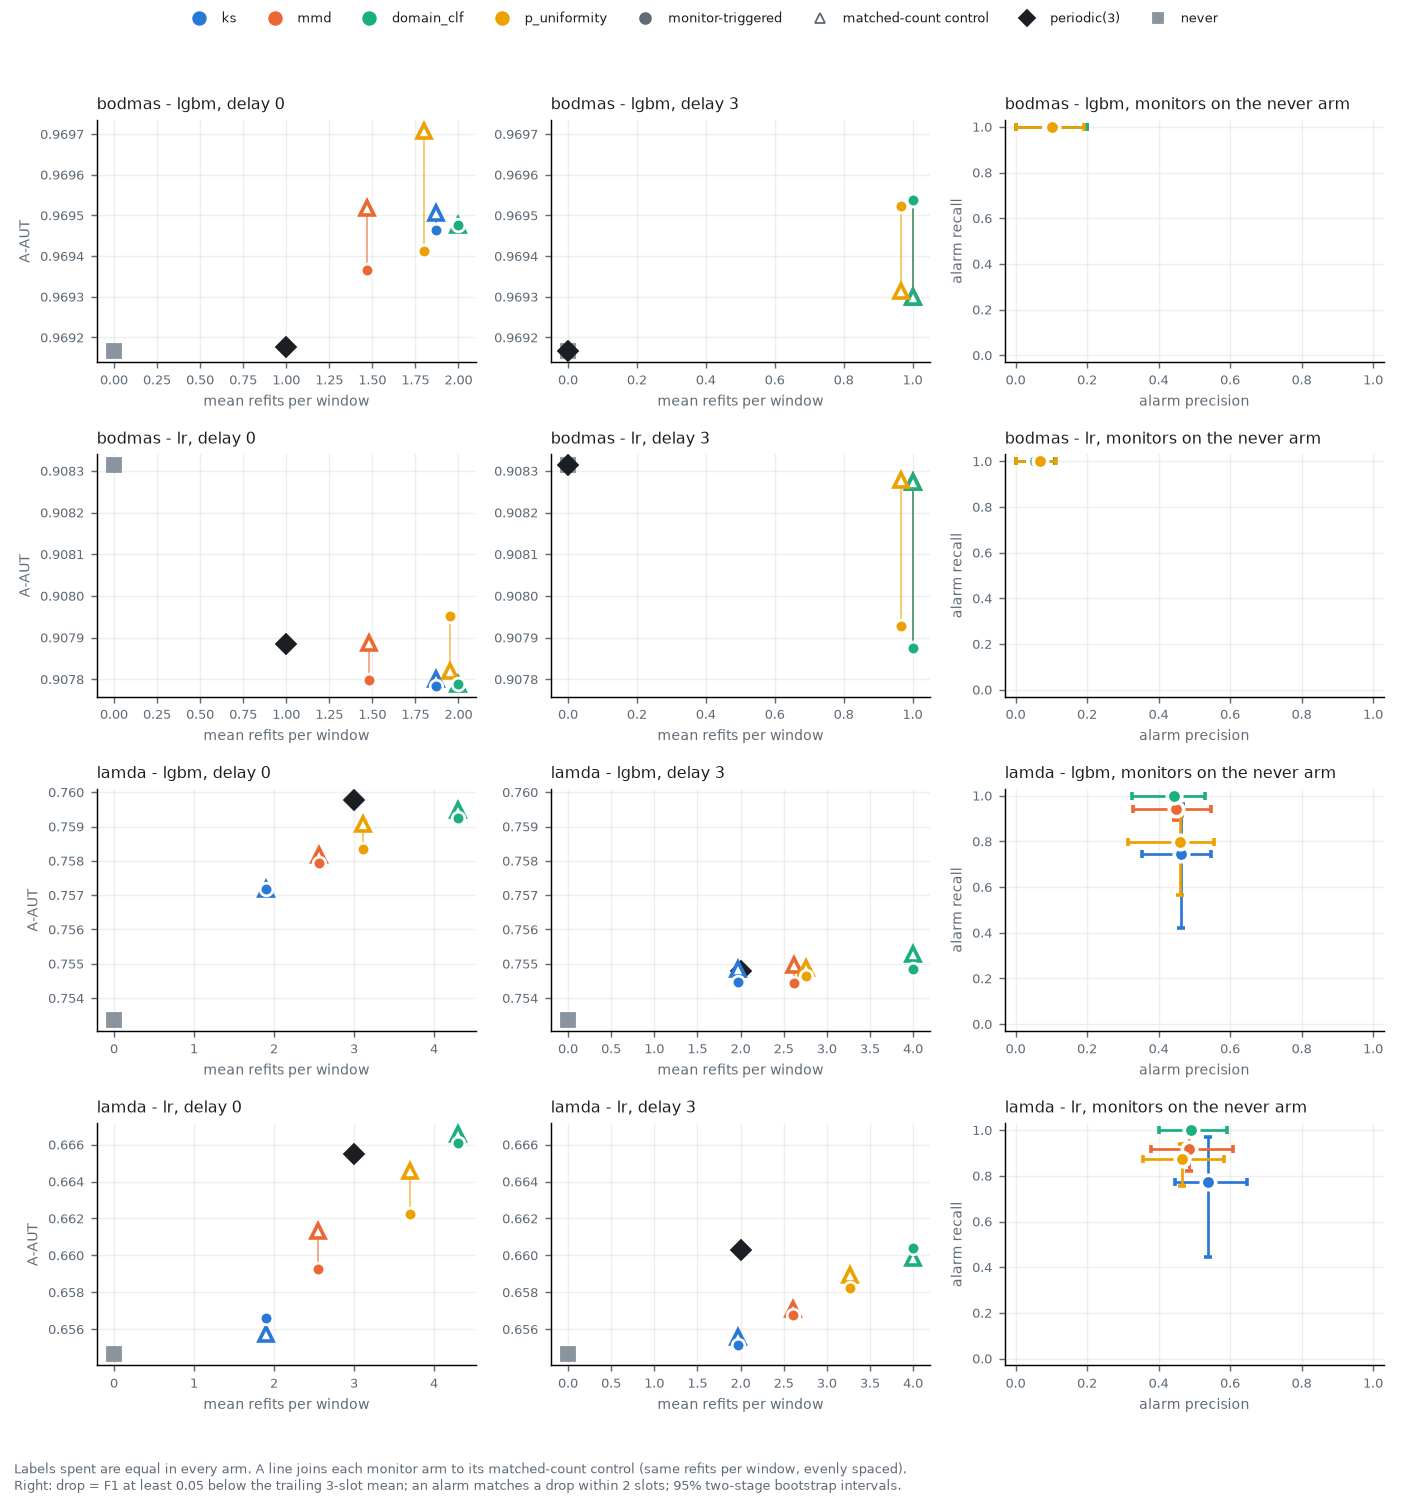
\includegraphics[width=0.92\textwidth]{../reports/figures/e4_monitors.png}
\caption{E4: A-AUT against mean refits per window for each monitor-triggered arm, its matched-count control, periodic retraining every third slot and never retraining, at delay 0 and 3 (left and middle columns), and alarm precision against recall for each monitor (right column). Labels spent are equal in every arm; intervals are two-stage bootstrap 95\% intervals.}
\label{fig:e4}
\end{figure*}

\section{Reading the results together}
Three observations hold across the four questions. First, the size of every effect is small next to the spread over windows, and the larger effects sit on LAMDA, the dataset with a longer series and more refit events per window; BODMAS offers one useful refit per window, so most of its contrasts are null or collapse into one comparison. Second, the label-selection result and the budget result are of the same order (about one to two hundredths of A-AUT), which suggests that at these budgets the choice of which labels to buy matters about as much as buying more, but the selector advantage is confounded with the class prior of the arrived labels: selection raises the malware share of the pool from 0.085 to between 0.19 and 0.40 on LAMDA (Table~\ref{tab:e3}), and a class-matched random baseline would separate the two effects. Third, the monitors alarm in most slots (alarm rates of 0.56 to 0.997 in Table~\ref{tab:e4}) and their precision stays near that of alarming every slot, so at the alarm level frozen before the run they are not informative about when to retrain; a different level, a larger sample per slot or a label-using monitor are untested.

\textbf{What was fixed before the results.} The window geometry and the size gate (ADR-0005), the metric thresholds (ADR-0006), the pool composition and the budget rule (ADR-0007), the E2 design and the RQ1 comparator (ADR-0008), the rule that calibration rows are never training rows (ADR-0009) and the monitor inputs and reference (ADR-0010) were decided and recorded in ADRs before the results of the grids they govern (E2 to E4), with the exception of the RQ1 comparator, which was chosen after E0 and E1 had been read. We emphasise this because the final conclusions are null or small: a null result is credible only if the analysis could not have been chosen to produce it.

\section{Threats to validity and limits}
\textbf{Small effects.} Effects are hundredths of A-AUT against window standard deviations of 0.05 to 0.07~\clm{E-28}; we do not claim that any of them matters operationally. \textbf{Few independent blocks.} LAMDA's 16 windows are about four independent blocks, seeds are draws of a subsample and not replicates of a model, so intervals are wide and their coverage was not measured~\clm{P-12}. The registered scheme resamples windows and then seeds within them; the statistical literature on hierarchical data favours resampling the top level only~\cite{davison1997bootstrap,ren2010hierarchical}, and our statement that the two-stage interval is wider rests on a synthetic check rather than on those sources.
\textbf{Labels.} LAMDA's labels are antivirus-centric and depend on a VirusTotal scan date the dataset does not publish, so a label may reflect later knowledge than the collection date, a leakage we cannot remove~\clm{D-16}. BODMAS's paper says families come mostly from multi-vendor antivirus verdicts analysed with in-house scripts and does not say how the binary label was decided~\cite{yang2021bodmas}.
\textbf{Class prior.} Per-slot F1 moves with the slot's malware share, correlating with the achieved ratio at 0.47 to 0.55 on LAMDA~\clm{E-66}, so part of the apparent decay is class prior; a prior-matched baseline and a threshold-free score are computable from stored predictions and were not registered.
\textbf{Simulated delay and analyst.} Delay is a whole number of slots, the same for every label, and a queried label is the dataset's truth returned without error. Neither dataset records when a label became known.
\textbf{One machine, two datasets, two detectors.} All runs are on one laptop, and a difference between datasets is not a finding about platforms.
\textbf{Review status.} The text has not yet been read line by line by a second person.

\section{Ethics and availability}
The work describes how detectors decay; it contains no malware, no decompiled code, no evasion tooling and no adversarial-example generation. Knowing when retraining pays could in principle help an adversary time an attack, but the study measures natural drift on public data, offers no method to cause drift and finds small effects.

\anonif{The code, the configurations, the claims ledger, the registrations, the decision records and the aggregate tables are in a public repository whose address is withheld for review. LAMDA, BODMAS and their licences are not redistributed; the repository holds only a synthetic fixture. Per-slot predictions are hashed in the repository and not yet deposited.}{The code (MIT), the configurations, the claims ledger, the registrations, the decision records and the aggregate tables are public at \url{https://github.com/Yathindra25KB/driftwatch-lifetime}. The package is \texttt{driftwatch-lifetime} on PyPI, and each release is archived on Zenodo (concept DOI 10.5281/zenodo.24050864). LAMDA, BODMAS and their licences are not redistributed; the repository holds only a synthetic fixture. Per-slot predictions are hashed in the repository and not yet deposited.}


\section{Conclusion}
Under one time-aware protocol with simulated delay, a fixed budget and four drift monitors, detector lifetime on LAMDA and BODMAS responds to retraining and to label timing by hundredths of A-AUT, selection by uncertainty or credibility adds a little over random selection and less after a delay, and no drift monitor beat retraining every third slot. The BODMAS series is too short to separate delay from refit counts. The contributions that outlast these numbers are the protocol, its assertions and audits, and a record in which every choice made before or after seeing results is labelled. Future work needs a new pre-registration each: other monitor settings, a longer BODMAS window, label noise and measured delay, a trap arm that also trains on released labels, class-prior controls, a registered lifetime measure, a label-using monitor, a cross-platform repeat and EMBER2024.

\bibliographystyle{IEEEtran}
\bibliography{references}

\end{document}
